
\subsection{SPI-in/PRBS}
This module only use basic leaf-cells at the transistor level, so this will be a quite small chapter. There are a few things worth noting regarding the sizing of these basic blocks. Some of the signals are connected to a large amount of devices (60+), which meant that the signal got really weak. This was solved by either just making the gates a bit bigger, or by using a buffer. SPI\_en is using a xx buffer, SPI\_clk is using a xx buffer, clk\_en is using a xx buffer and test\_mode is using a 9x buffer.

\subsection{16-bit Kogge-Stone Adder}
The Kogge-Stone adder consists of four simple blocks connected in a complex way, as can be seen in \ref{app:ks_block}. These four blocks can be seen in figure \ref{fig:red}-\ref{fig:sum}. The red block constitute the initial stage which takes two binary numbers $A$ and $B$ as input. The corresponding truth table is found in table \ref{tab:red} in appendix \ref{app:ks_truth}. The output signals $P$ and $G$ generated from this block are later used by other blocks in the adder. The $G$, also called the Generate signal, trickles down through the hierarchy of yellow, and yellow carry blocks to finally end up in the sum block. The truth table for this block can be found in table \ref{tab:sum}. Truth tables for the yellow and yellow carry blocks are found in table \ref{tab:yellow} and \ref{tab:yellowcarry}.

\begin{figure}[H]
  \centering
  \captionsetup{justification=centering}
  \adjustbox{trim={.3\width} {0\height} {.3\width} {0\height},clip}
  {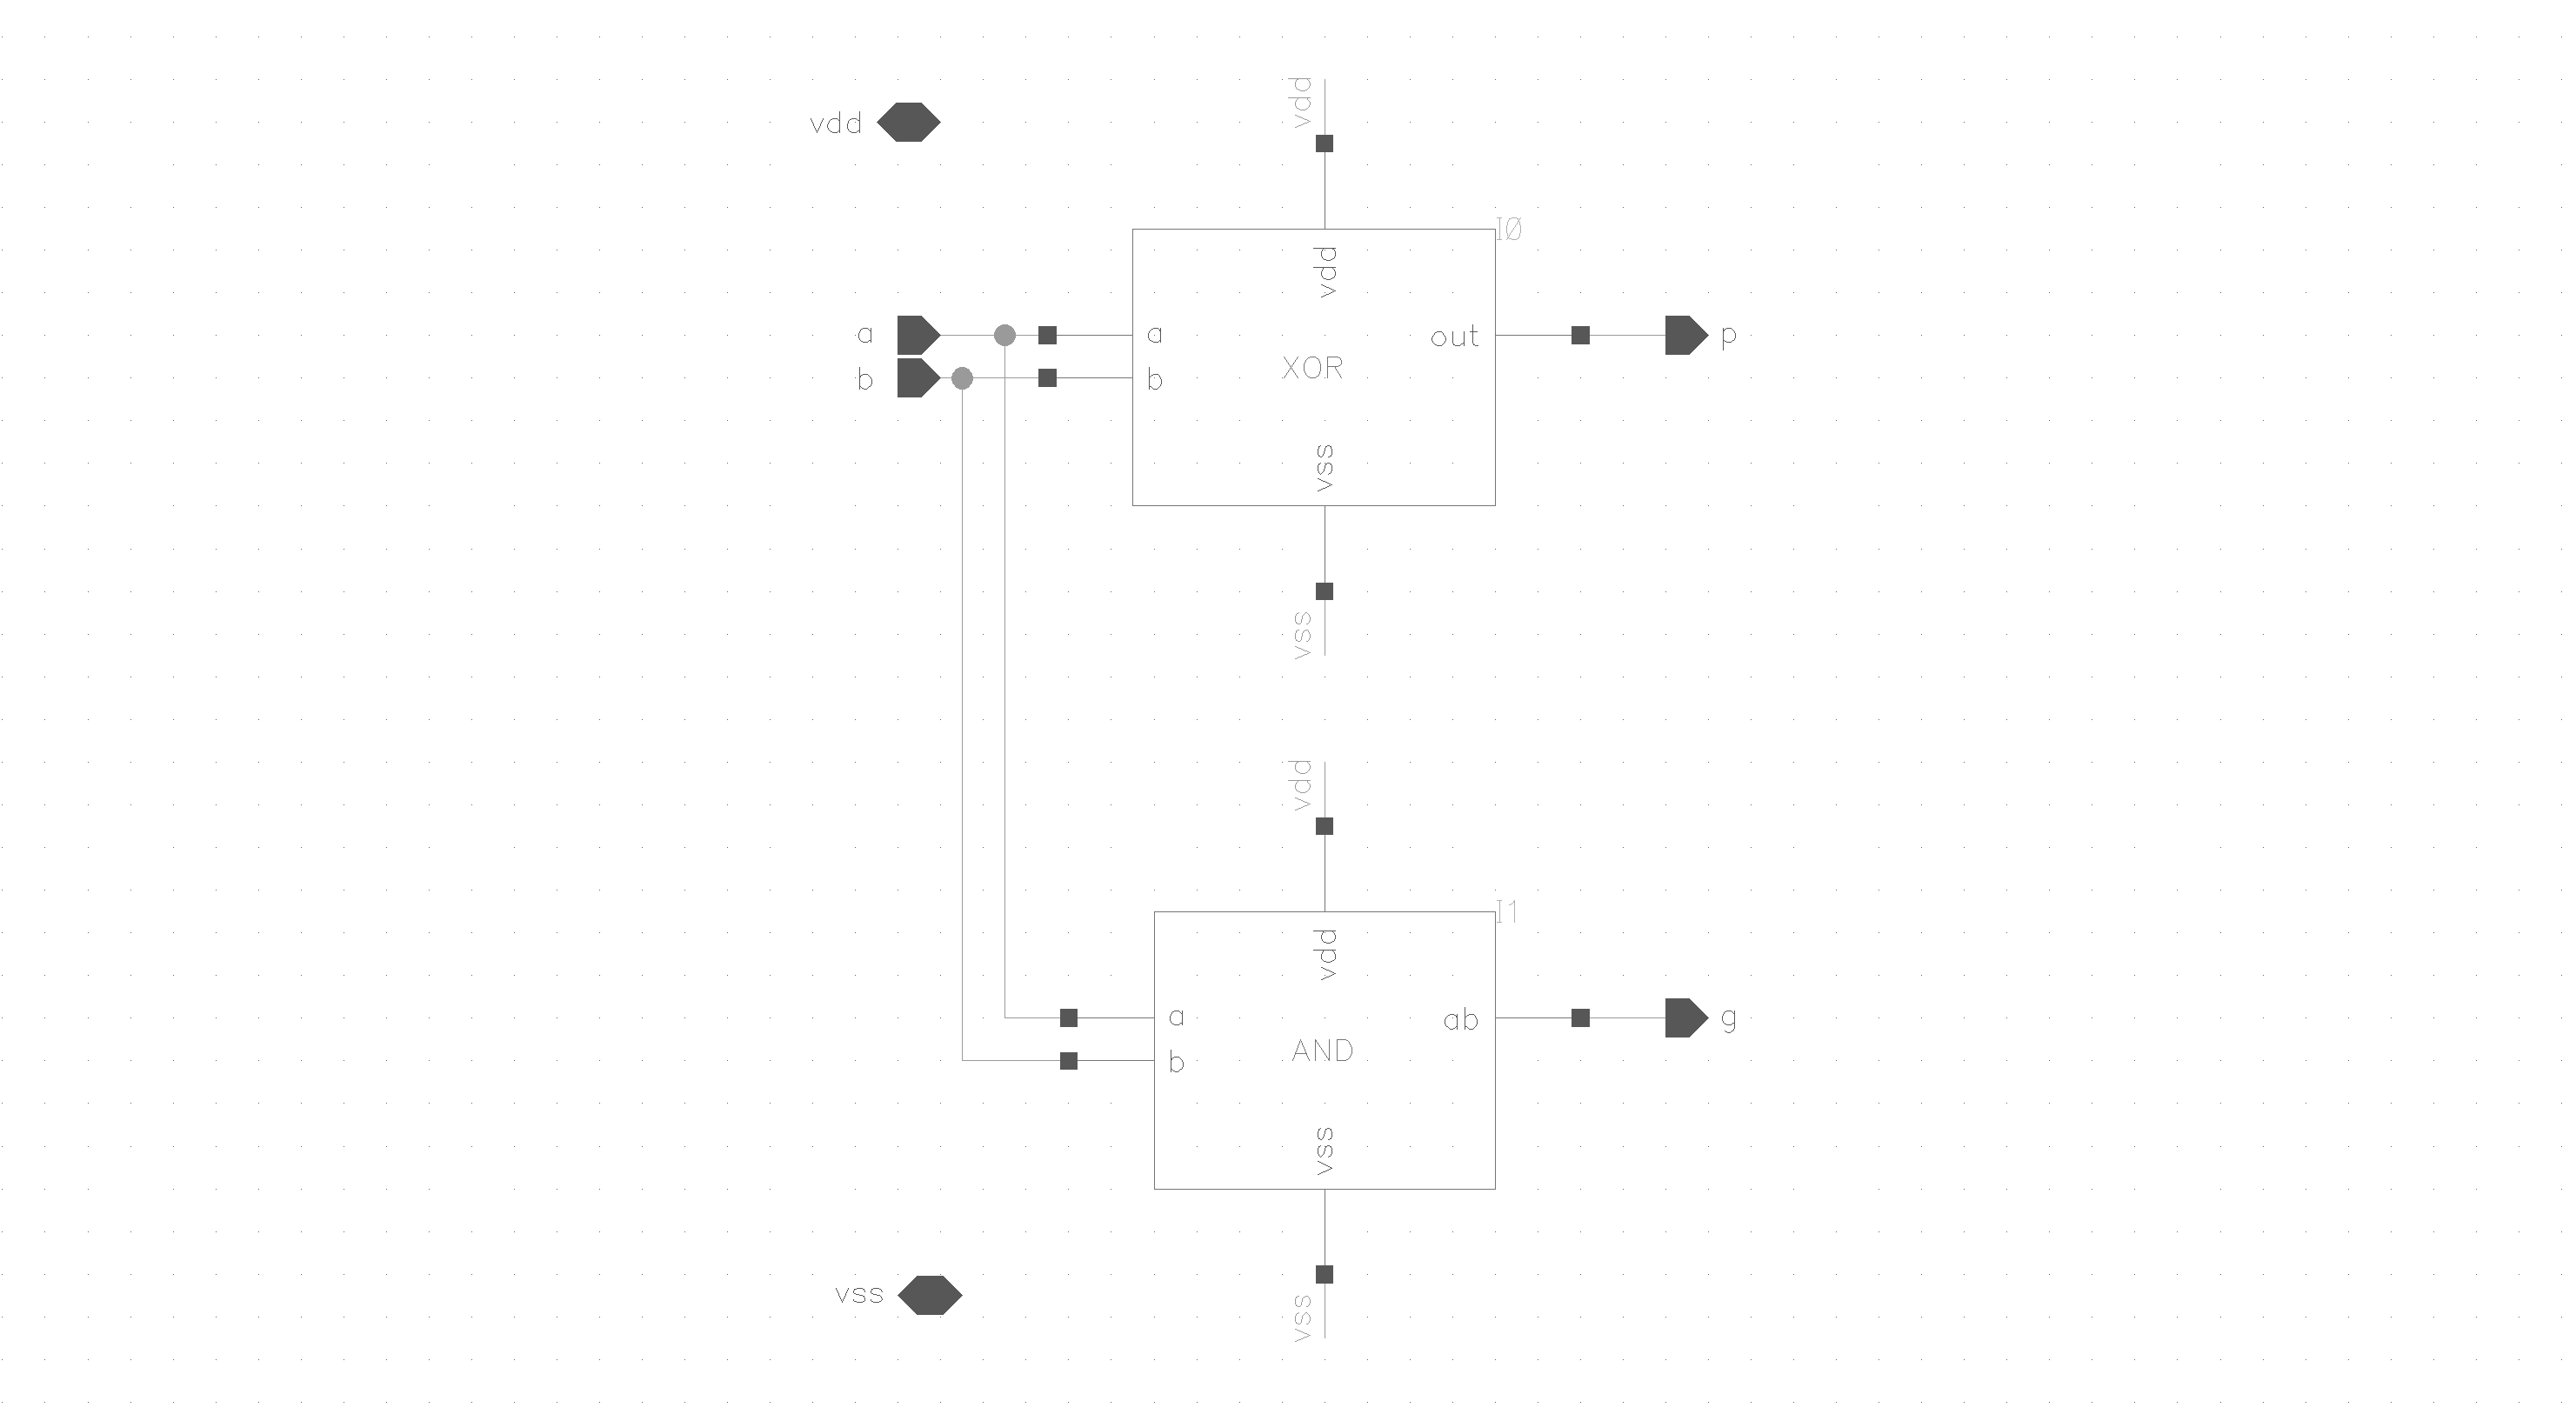
\includegraphics[width=2.0\textwidth]{../figures/red}}
  \caption{Schematic view of the red block.} \label{fig:red}
\end{figure}

\begin{figure}[H]
  \centering
  \captionsetup{justification=centering}
  \adjustbox{trim={.15\width} {0\height} {.12\width} {0\height},clip}
  {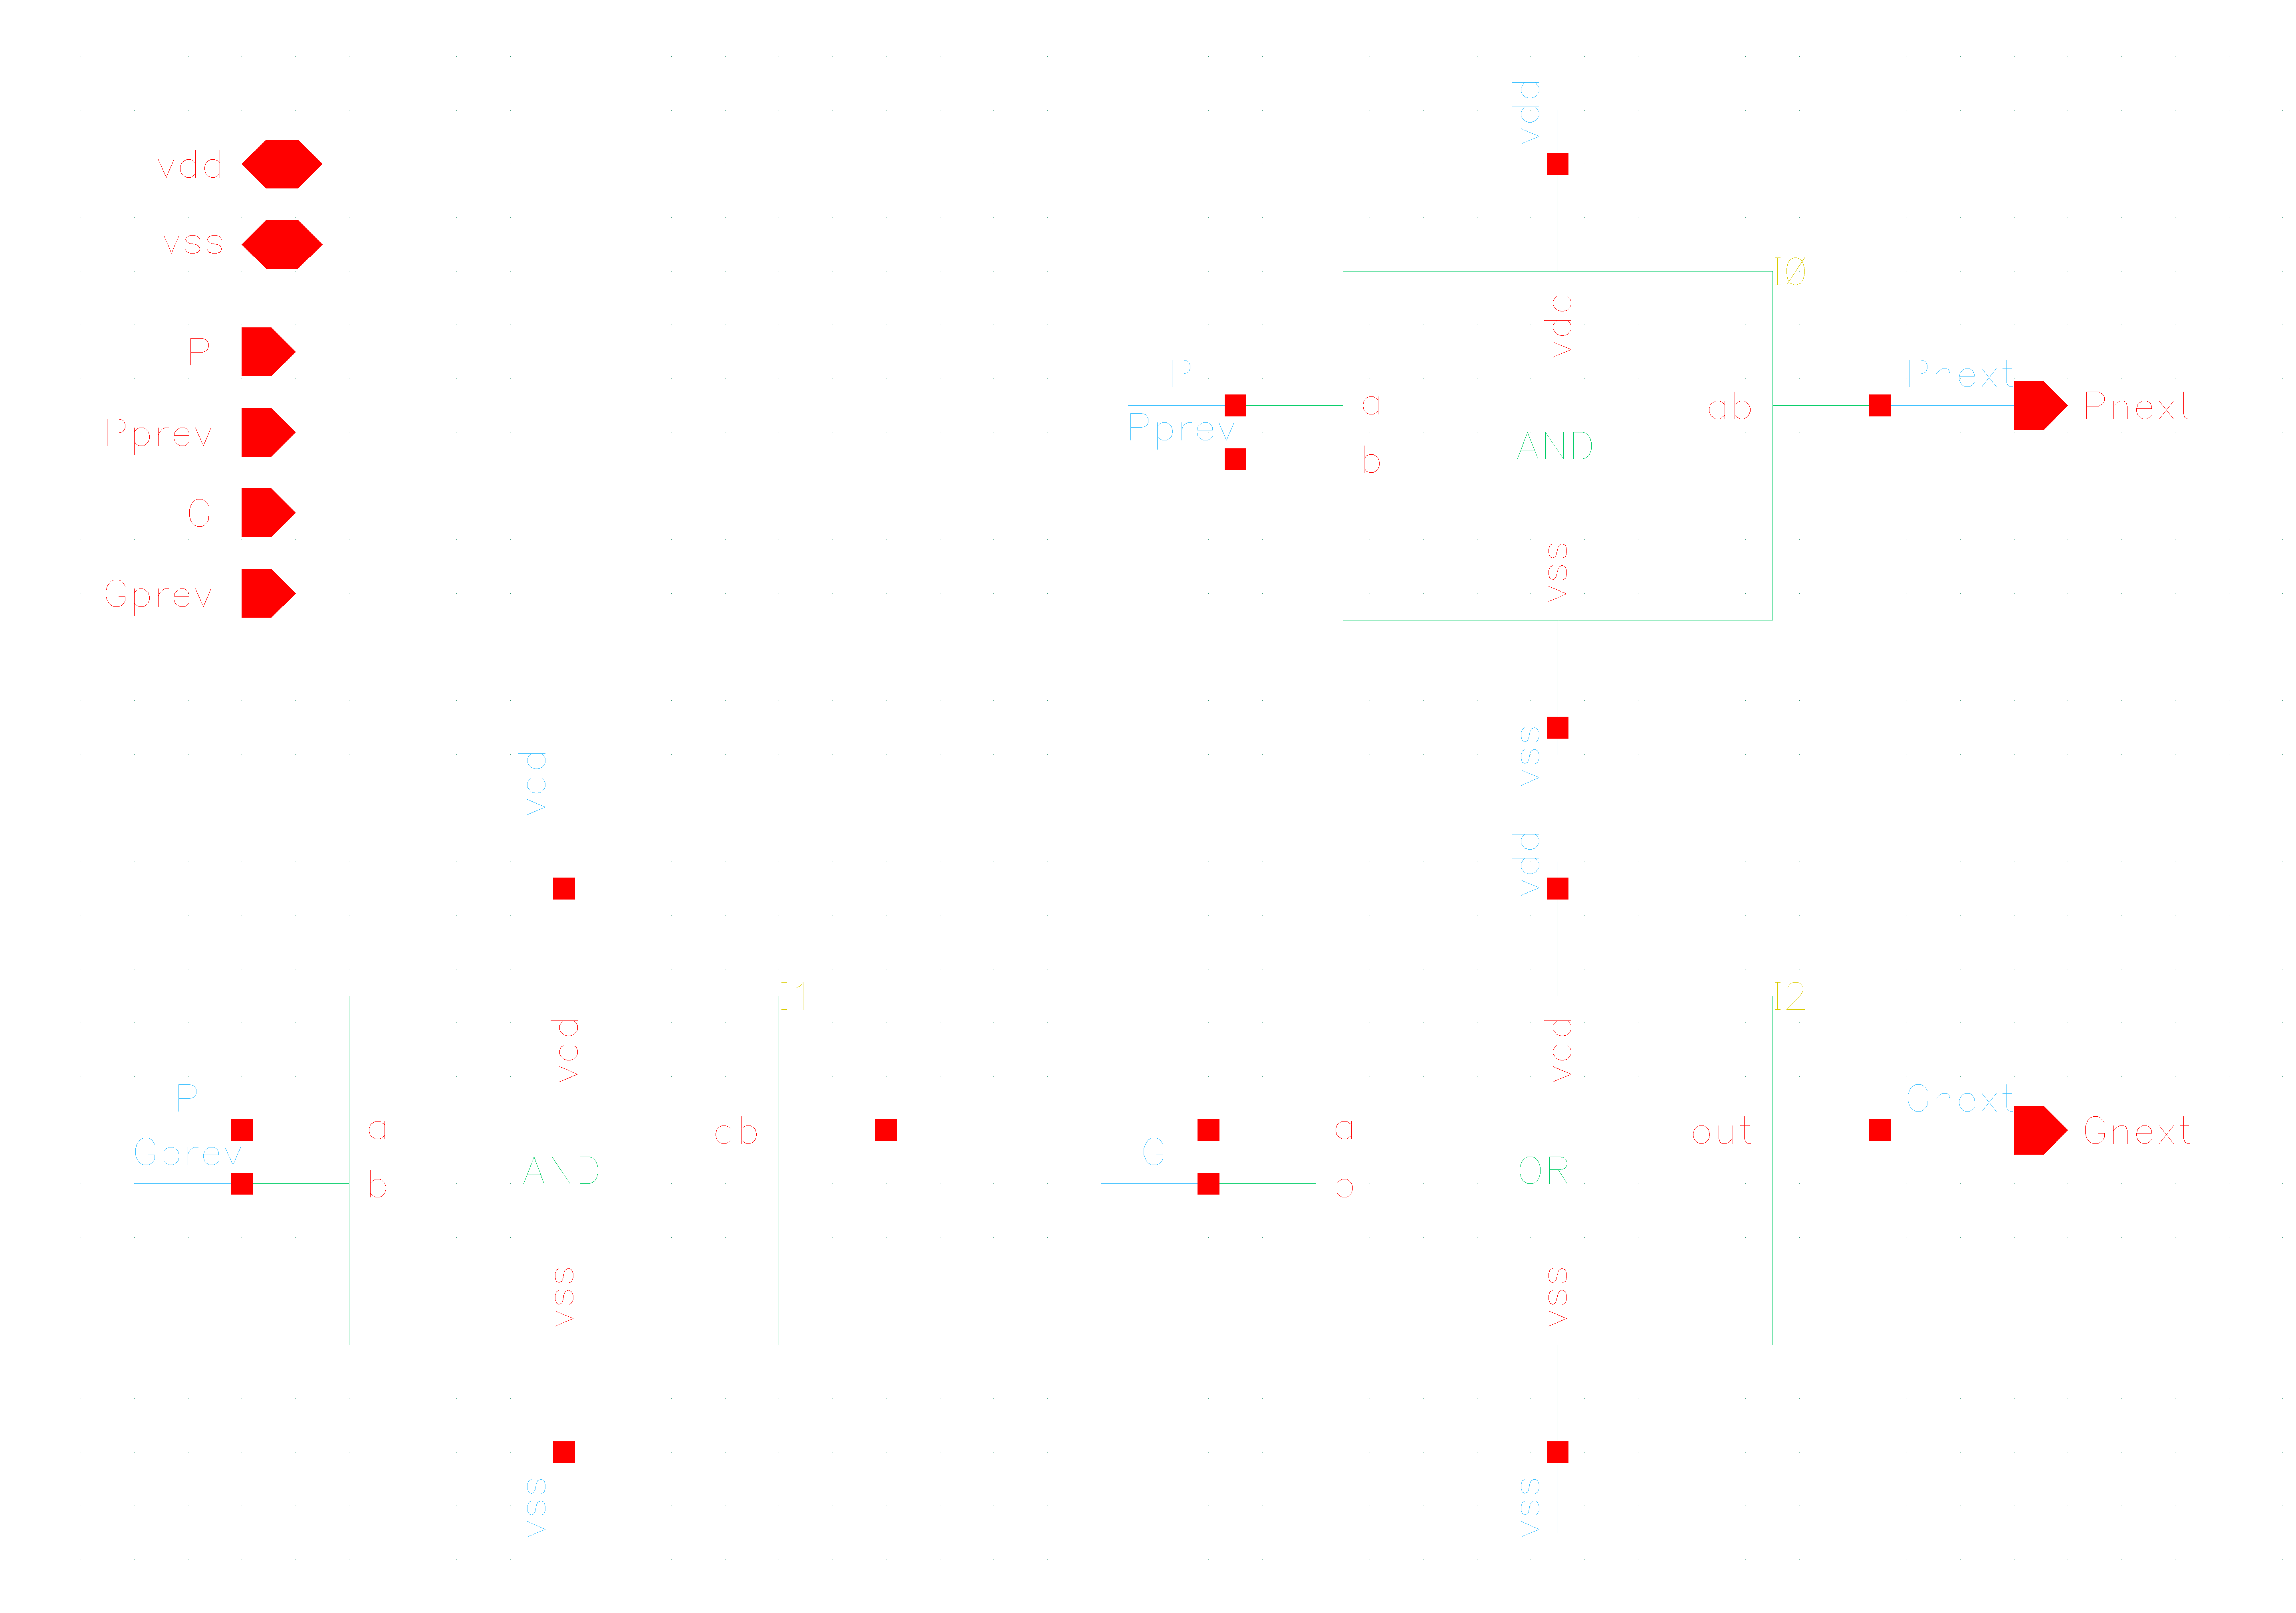
\includegraphics[width=1.3\textwidth]{../figures/yellow}}
  \caption{Schematic view of the yellow block.} \label{fig:yellow}
\end{figure}

\begin{figure}[H]
  \centering
  \captionsetup{justification=centering}
  \adjustbox{trim={.1\width} {0\height} {.1\width} {.4\height},clip}
  {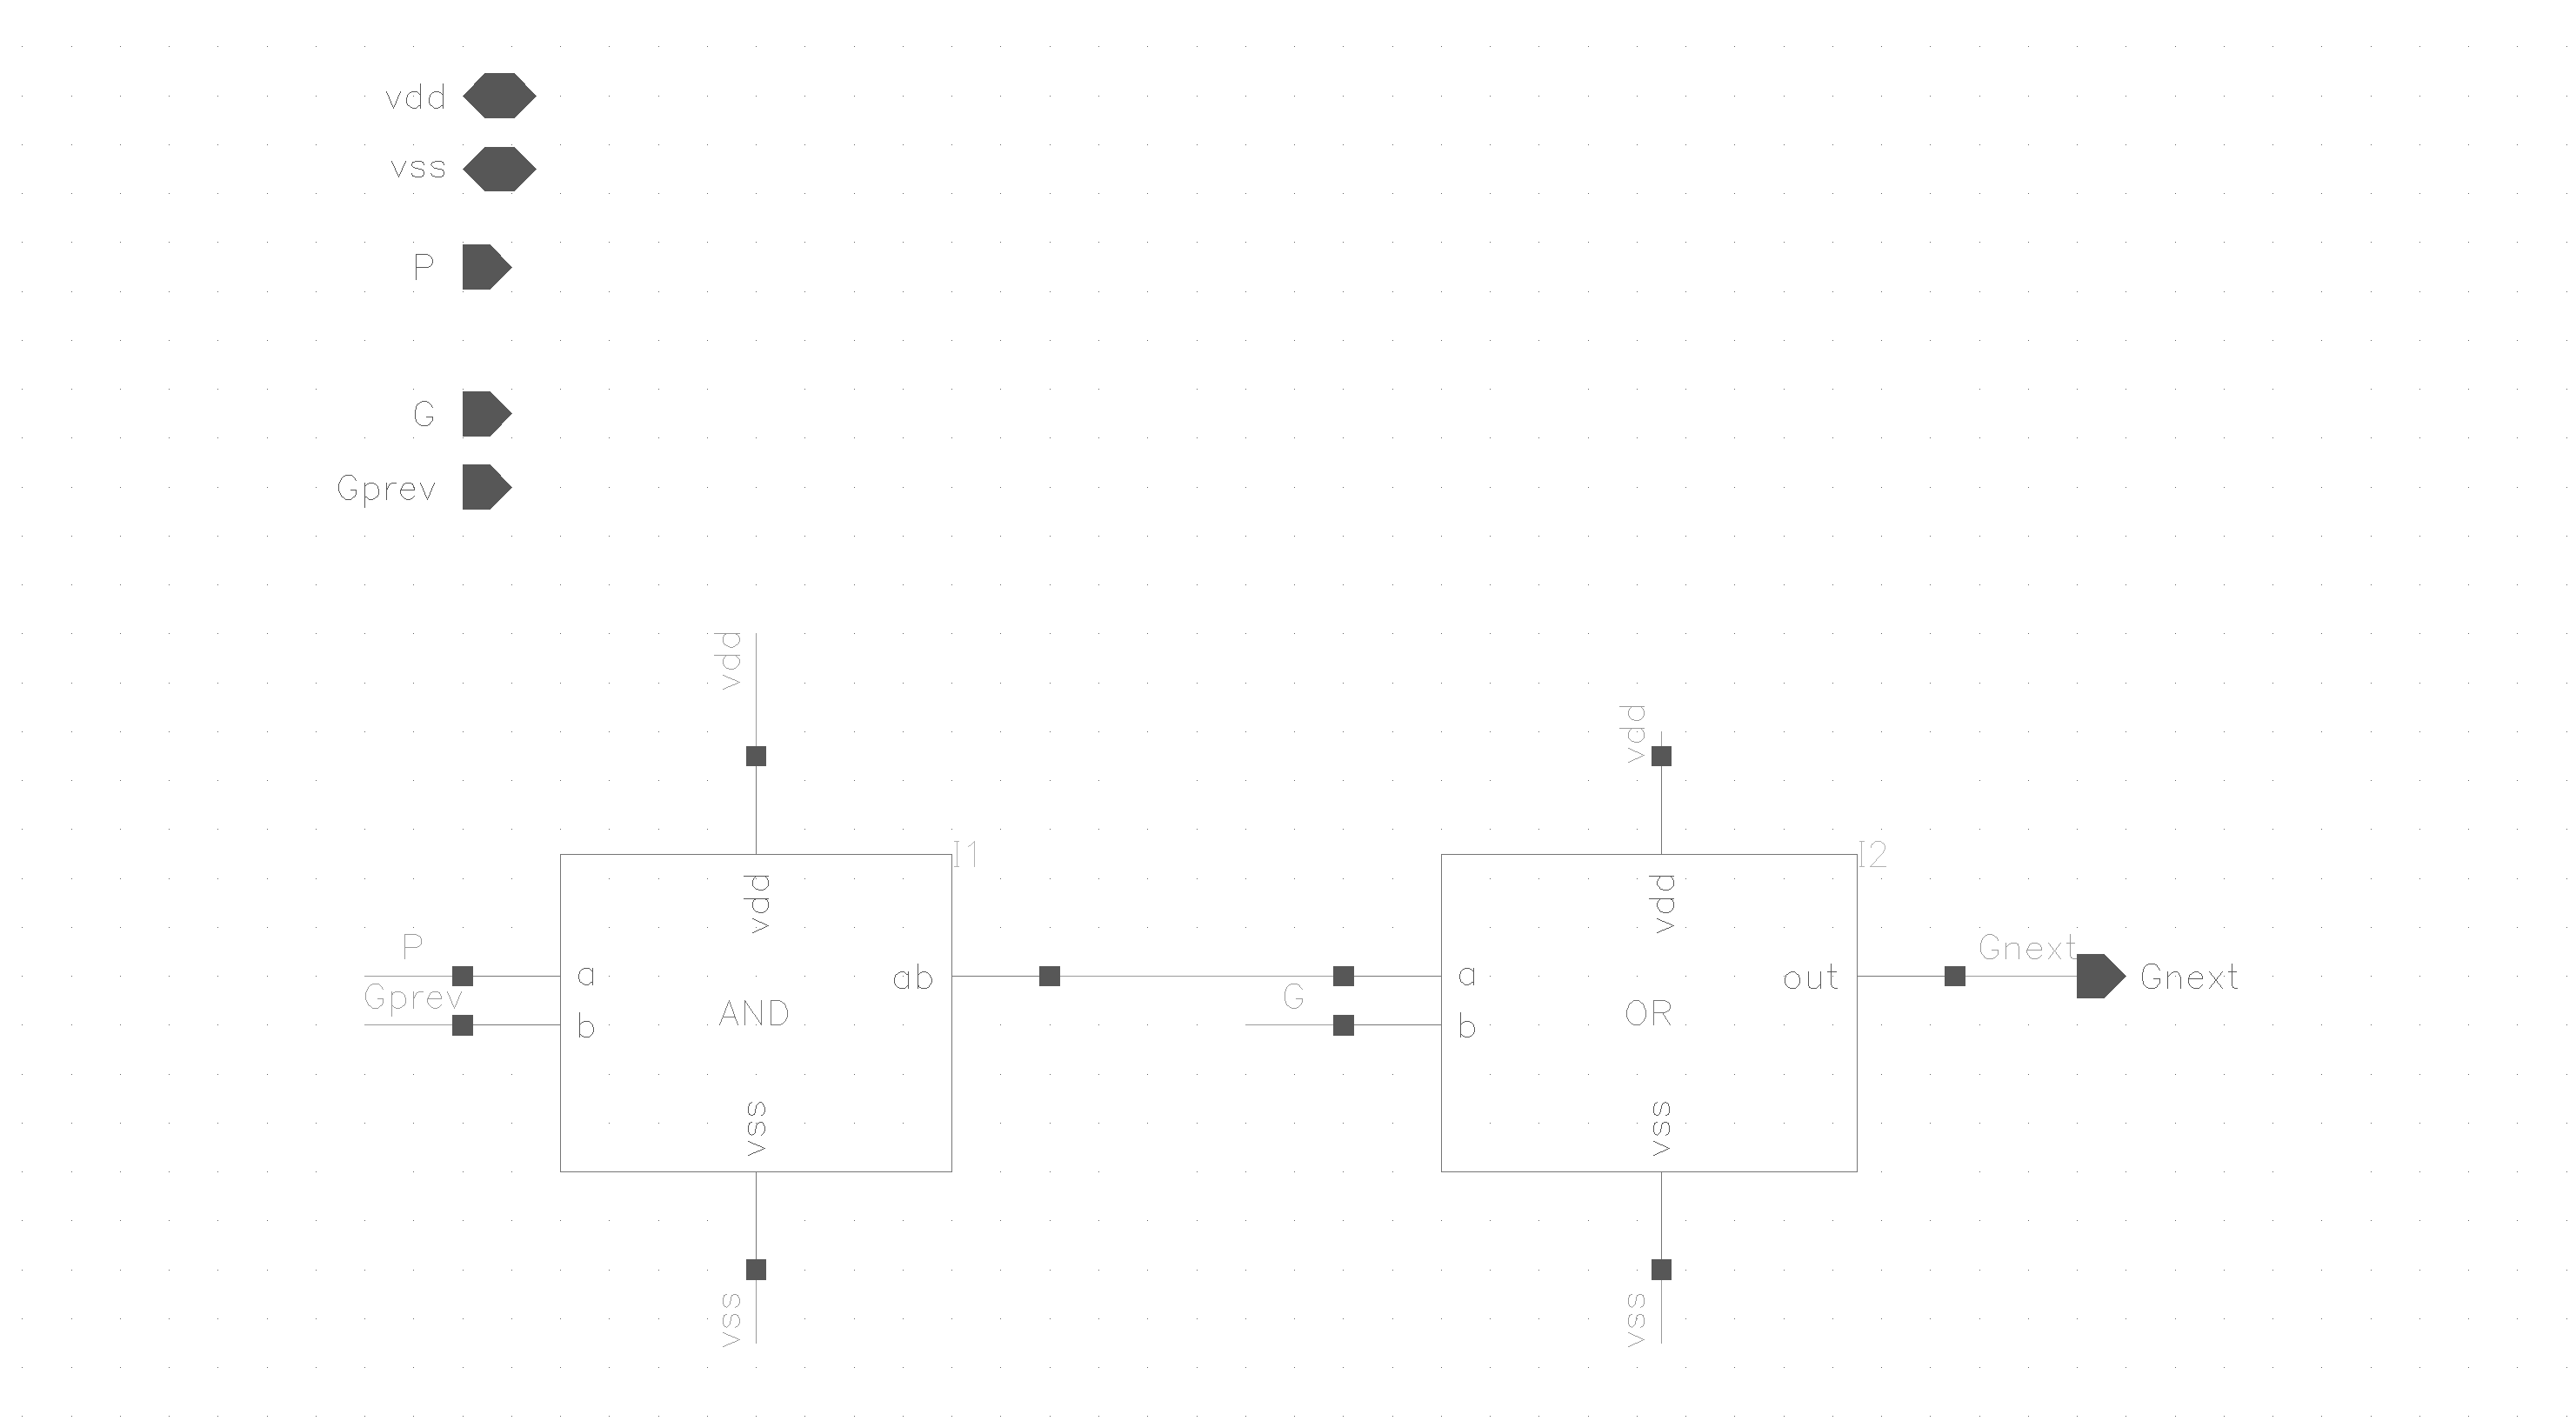
\includegraphics[width=1.2\textwidth]{../figures/yellow_carry}}
  \caption{Schematic view of the yellow carry block.} \label{fig:yellow_c}
\end{figure}

\begin{figure}[H]
  \centering
  \captionsetup{justification=centering}
  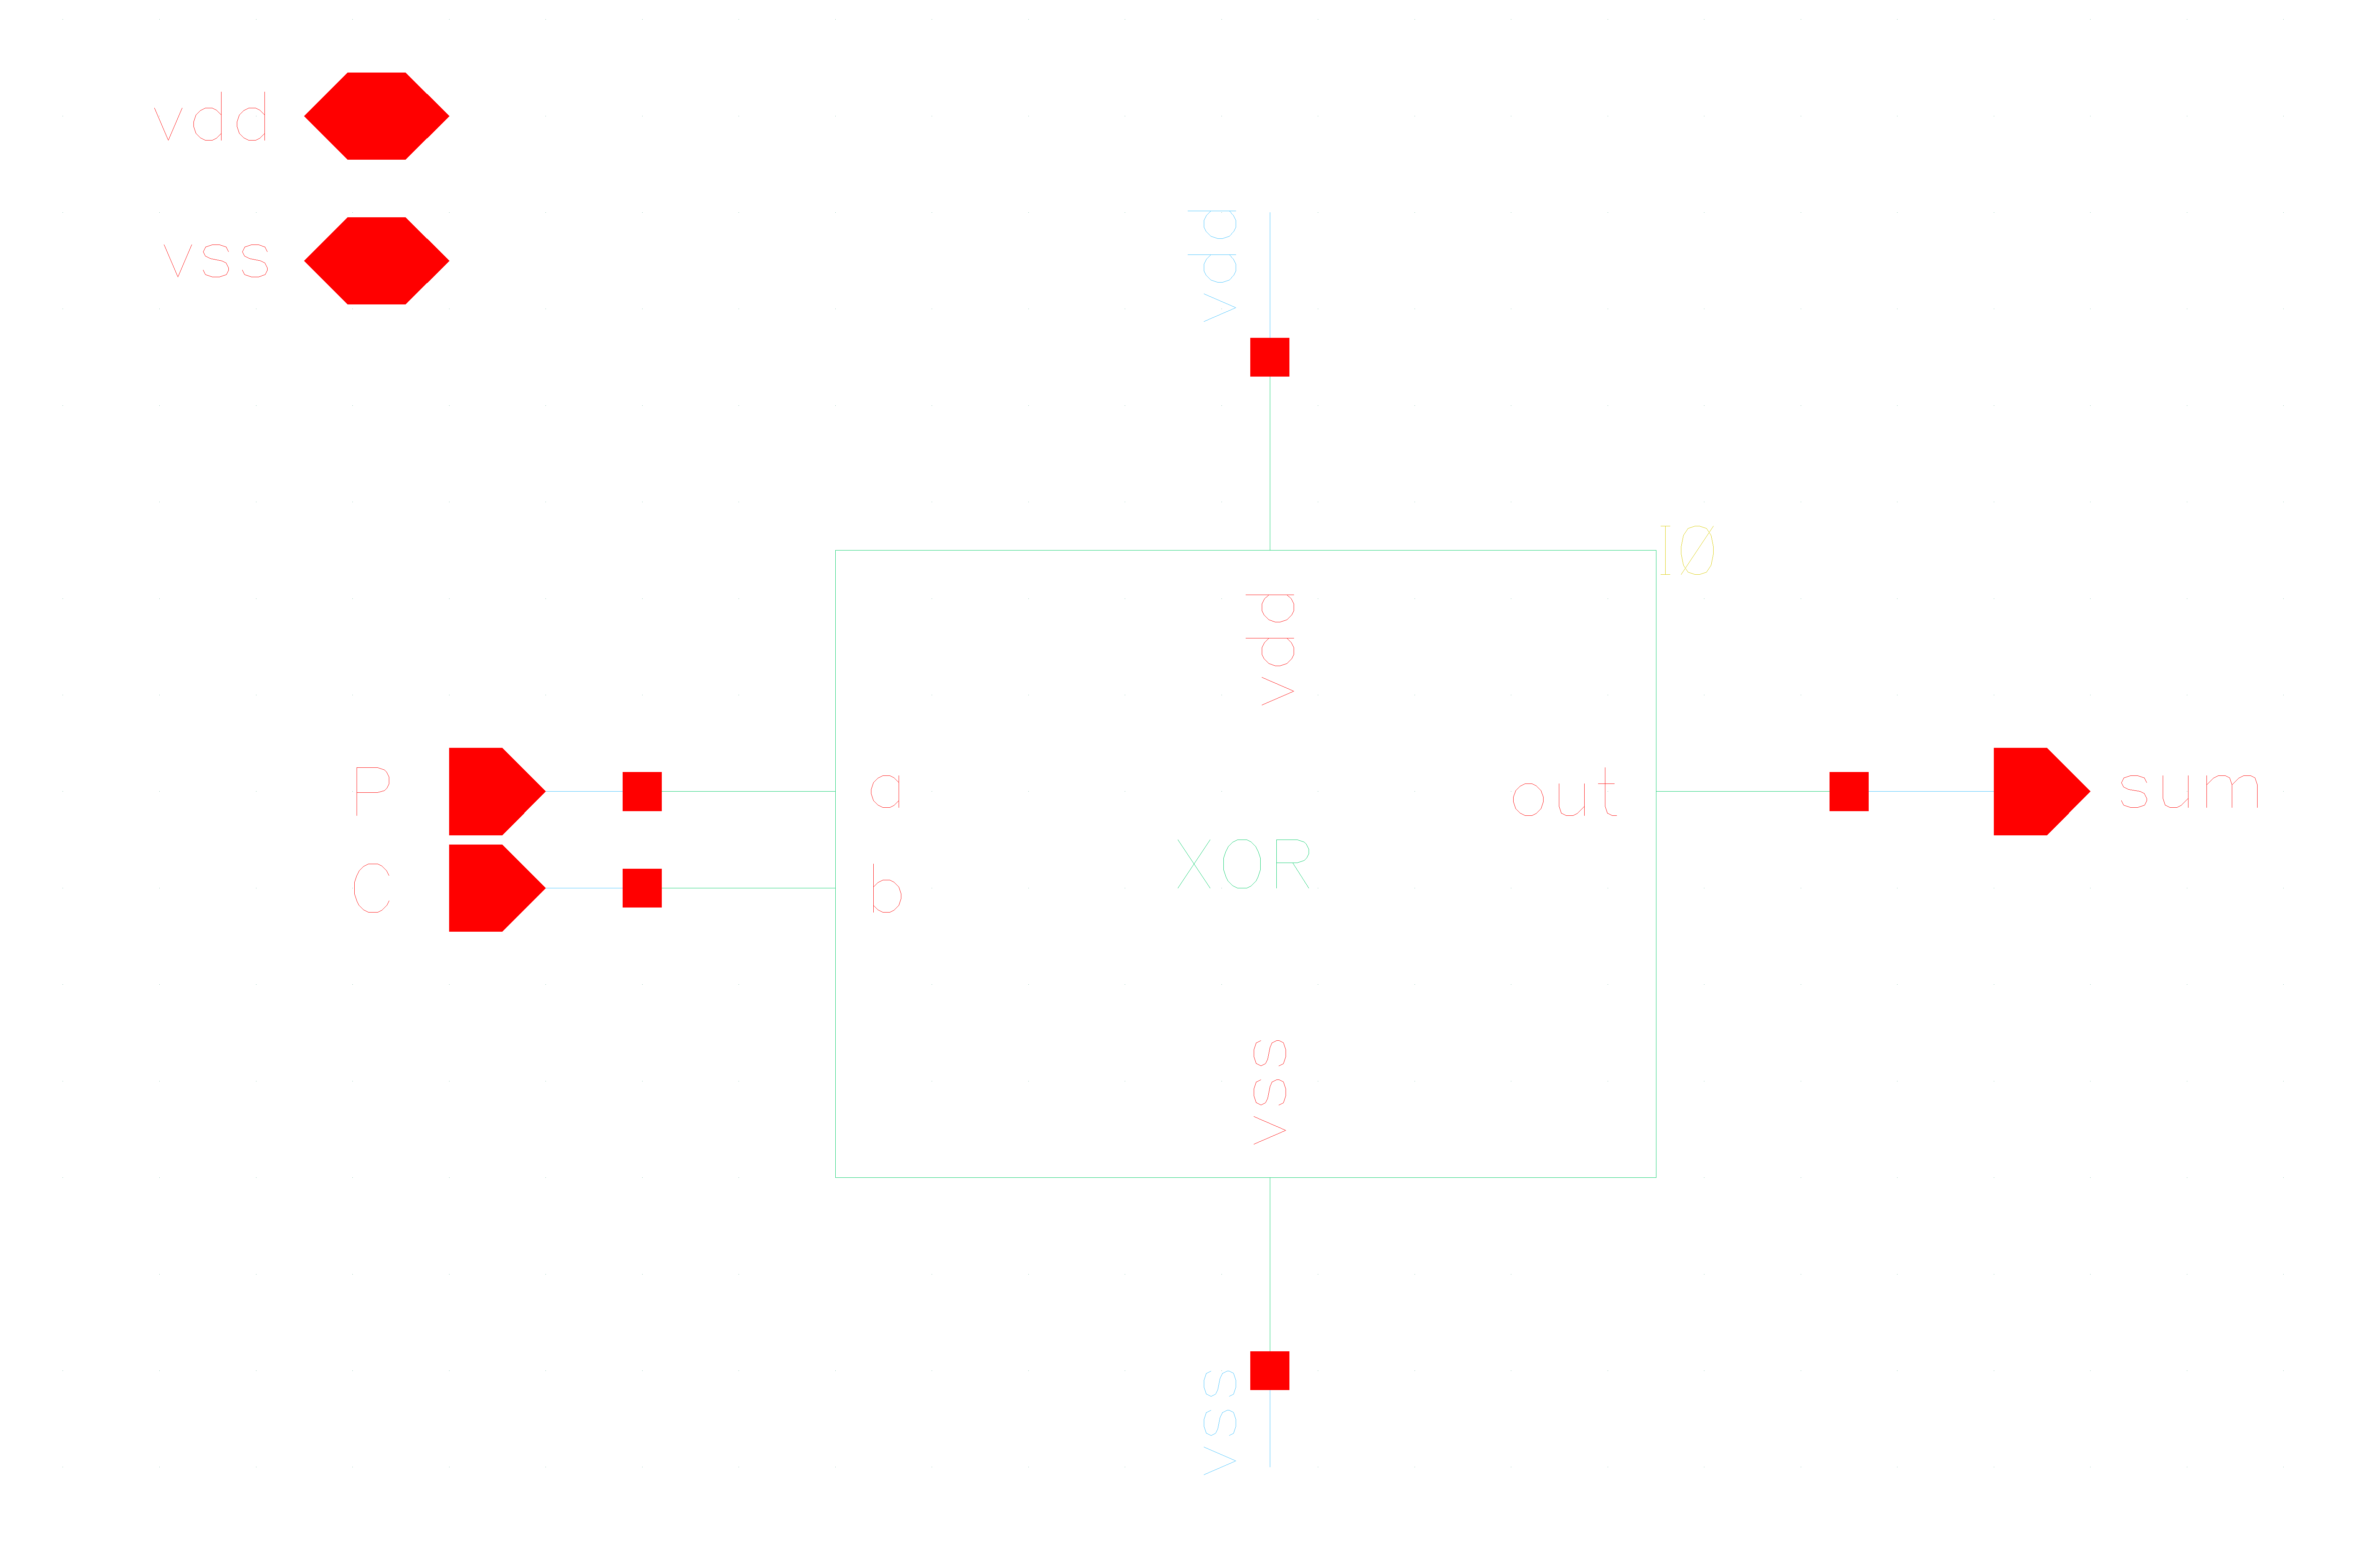
\includegraphics[clip,width=1.0\textwidth]{../figures/sum}
  \caption{Schematic view of the sum block.} \label{fig:sum}
\end{figure}

\subsection{Comparator}
The comparator consists of 17 2-input XNOR gates where one bit of each number is fed into each gate. The output from the XNOR gates are fed into a couple of AND gates which generates the final output. The comparator is 17 bits wide since it compares two 16 bit numbers plus their carry bits. The logic table of the XNOR gates is shown in table \ref{tab:xnor}.

\begin{table}[H]
  \caption{Logic table of XNOR block.}
  \centering
  \begin{tabular}{cc|c}
    \toprule
    $A_i$ & $B_i$ & $Y = \overline{(A_i \oplus B_i)}$ \\
    \midrule
    0 & 0 & 1 \\
    0 & 1 & 0 \\
    1 & 0 & 0 \\
    1 & 1 & 1 \\
    \bottomrule
    \label{tab:xnor}
  \end{tabular}
\end{table}
